\documentclass[../AP_Statistics.tex]{subfiles}

\begin{document}
	\chapter{One-Variable Quantitative Data}
		Statistics is the science of collecting and analyzing data. \\
		A data set is a collection of data on several \textbf{individuals}. These individuals can be anything. \\
		Data provides values for \textbf{variables}, which describe some characteristic of an individual. \\
		A variable's \textbf{distribution} describes the frequency with which a variable takes on its possible values.
		\section{Graphically Displaying Distributions}
			Quantitative variables can either be \textbf{discrete}, having some countable set of possible values, or \textbf{continuous}, having an uncountable set of possible values.
			\callout{17}{The quantitative variable being described must always be defined, typically as a capital letter. An arbitrary particular value is denoted with a lowercase letter and a superscript is added to denote a defined value.}
			\textbf{Dot plots} assign the horizontal axis to the variable and show each value's frequency with a number of dots above, each corresponding to an individual. \\
			\textbf{Stem (and leaf) plots} can only display quantities. The stem (vertical axis) corresponds to the first digit while the leaf (horizontal axis) corresponds to the remaining digits. The stem is always on the left, and the leaves should always be ordered from least to greatest. A key is required to denote the magnitudes displayed. \\
			\textbf{Histograms} show bars that are assigned equal intervals. To find the length of each interval, the range can be divided by the number of classes and the result rounded up. Each bar's height shows the number of individuals within the class. \\
			\textbf{Time plots} measure a variable over time. \\
			A \textbf{cumulative frequency curve} (OGIVE) is a line graph that shows the cumulative relative frequency, the sum of all lower classes' \textbf{relative frequencies}, the percentages of data contained within each class, (inclusive). Rather than each class being represented as a range, they are labeled by their medians.
			\subsection*{Graphically Describing Distributions}
				A distribution can be described by its shape, outliers, center, and spread (SOCS).
				\paragraph{Shape}
					In order for a distribution to be symmetric, values that are equidistant from the mode must have the same frequencies. \\
					\begin{center}
						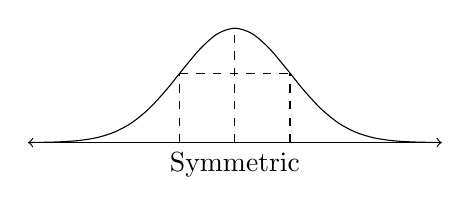
\begin{tikzpicture}[xscale = 0.7, yscale = 3.64]
							\draw[<->] (-3.75, 0) -- node[below]{Symmetric} ++ (7.5, 0);
							\draw[domain = -3.75:3.75, smooth, variable = \x] plot({\x}, {e^(-0.5 * \x * \x)/sqrt(2 * pi)});
							\draw[dashed] (0, 0) -- (0, 0.399);
							\draw[dashed] (-1, 0) -- (-1, 0.242);
							\draw[dashed] (1, 0) -- (1, 0.242);
							\draw[dashed] (-1, 0.242) -- (1, 0.242);
						\end{tikzpicture}
					\end{center} 
					\textbf{Skew} is dependent on whether the tail is on the direction of the tail.
					\begin{align*}
						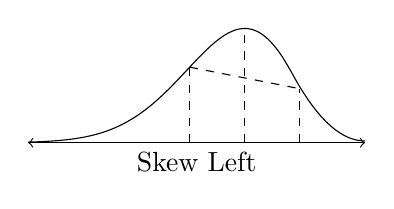
\begin{tikzpicture}[yscale = 2]
							\draw[<->] (-3.75, 0) -- node[below] {Skew Left} ++ (4.278, 0); 
							\draw[domain = -3.75:-0.4, smooth, variable = \x] plot({\x}, {((e^(-0.5 * \x * \x))/sqrt(2 * pi)) * -3 * \x});
							\draw[domain = -0.4:0.528, smooth, variable = \x] plot({\x},{0.5*\x*\x - 0.528 * \x + 0.1508});
							\draw[dashed] (-1, 0) -- (-1, 0.726);
							\draw[dashed] (-1.7, 0) -- (-1.7, 0.48);
							\draw[dashed] (-0.3, 0) -- (-0.3, 0.343);
							\draw[dashed] (-1.7, 0.48) -- (-0.3, 0.343);
						\end{tikzpicture}
						&&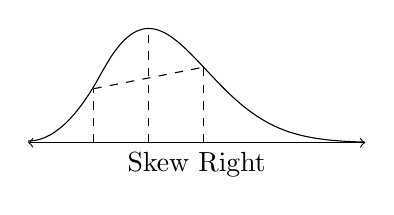
\begin{tikzpicture}[yscale = 2]
							\draw[<->] (-0.528, 0) -- node[below] {Skew Right} ++ (4.278, 0);
							\draw[domain = 0.4:3.75, smooth, variable = \x] plot({\x}, {((e^(-0.5 * \x * \x))/sqrt(2 * pi)) * 3 * \x});
							\draw[domain = -0.528:0.4, smooth, variable = \x] plot({\x},{0.5*\x*\x + 0.528 * \x + 0.1508});
							\draw[dashed] (1, 0) -- (1, 0.726);
							\draw[dashed] (0.3, 0) -- (0.3, 0.343);
							\draw[dashed] (1.7, 0) -- (1.7, 0.48);
							\draw[dashed] (0.3, 0.343) -- (1.7, 0.48);
						\end{tikzpicture}
					\end{align*}
				\paragraph{Outliers}
					An \textbf{outlier} is a point that does not fit the general trend of the data. It is marked as an asterisk on a modified box plot. \\
				\paragraph{Center}
					The mean ($\bar{x}$), median ($Q_2$), and mode are measures of center. The relationship between these quantities is related to the skew.
					\[\begin{array}{|c|ccc|}\hline
						\rm{Skew} & \rm{Left} & \rm{Center} & \rm{Right} \\\hline
						\rm{Relationship} & \bar{x} < Q_2 < \rm{mode} & \bar{x} = Q_2 = \rm{mode} & \bar{x} > Q_2 > \rm{mode} \\\hline
					\end{array}\]
				\paragraph{Spread}
					The standard deviation, range, and interquartile range are measures of spread, The greater they are, the more variability there is in the data.
		\section{Numerically Describing Distributions}
			The \textbf{mean} is the sum of each value (not necessarily unique) in the distribution divided by the total number of values. It is also referred to as the average or expected value of its variable. For a sample, it is denoted using a bar over the lowercase form of its variable ($X$ becoming $\bar{x}$).
			\[\bar{x} = \frac{\sum x_i}{n}\]
			The first, second, and third \textbf{quartiles}, denoted $Q_1$, $Q_2$, and $Q_3$, are the values with 25\%, 50\%, and 75\% of the data below them respectively.\footnote{The probability of $X$ falling below each quartile is equal to its number multiplied by 25\%. \begin{align*} P(X < Q_1) &= 0.25 & P(X < Q_2) &= 0.5 & P(X < Q_3) &= 0.75\end{align*}} The second quartile is the \textbf{median}. \\
			The \textbf{mode} is the value that appears with the greatest frequency. It is, along with the mean and median, a measure of center. \\
			The \textbf{range} is the difference between the highest and lowest values of a data set. \\
			The \textbf{interquartile range}, denoted $IQR$, is the difference between the values of the third and first quartiles.\footnote{A box plot shows the interquartile range as the box and the median as the line within it.} It therefore shows the \enquote{middle half} of the distribution.
			\[IQR = Q_3 - Q_1\]
			The \textbf{standard deviation} is the average distance from the mean. It is denoted by $s$  with the subscript of its variable's lowercase form (for a sample). Along with the range and interquartile range, it is a measure of spread/variability.
			\[s_x = \sqrt{\frac{\sum (x_i - \bar{x})^2}{n - 1}}\]
			\callout{17}{It is crucial to note that the mean and standard deviation are only to be used when there are no outliers\footnote{An \textbf{outlier} is any value that varies from the middle 50\% by over 1.5 multiplied by the interquartile range. \[(|Q_1 - x_i| \lor |x_i - Q_3|) > 1.5IQR \implies x_i \text{ is an outlier}\]} due to their sensitivity.}
			The \textbf{variance} is the square of the standard deviation and is accordingly denoted by $s^2$ with the appropriate subscript. \footnote{The values of $n$, $\sum x_i$, $\bar{x}$, $Q_1$, $Q_2$, $Q_3$,  range, $IQR$, $s_x$, and $s_x^2$ are all calculable automatically given a data set. The data can be entered into $\texttt{L}n$ ($\texttt{Stat/EDIT/1}$), and $\texttt{1-Var Stats}$ ($\texttt{Stat/CALC/1}$) can be performed with $\texttt{L}n$ ($\texttt{ALPHA/}n$) as its parameter.} \\
			A \textbf{linear transformation} shifts all values by the same amount $a$ and/or proportionally to their values (with constant of proportionality $b$), resulting in a new variable. 
			\[y_i = a + bx_i\]
			It should be noted that the measures of center are changed by both $a$ and $b$, but only the former alters the measures of spread.
		\section{Density Curves}
			A \textbf{density curve}, typically denoted $f$, displays the \enquote{relative frequencies} of every possible value of its variable. As such, the total area under the curve must be exactly 1 and its values must always be positive. \\ 
			A density curve is a \textbf{continuous} distribution, so the probability of $X$ being any particular value is 0.\footnote{Probability is equal to the integral over the desired interval, so when both bounds are the same, it will be equal to zero.\[\int_x^xf(t)\,dt = F(x) - F(x) = 0\]}
			\callout{17}{Because the probability of $X$ being any particular value is 0, the function's output values do not actually represent anything, though they can be compared to the relative frequencies of distribution curves.}
			Because a density curve is effectively an idealized distribution curve, representing a population rather than a sample, different variables are used. \\ 
			\[\begin{array}{|c|c|c|}\hline
				\rm{Value} & \text{Sample Data} & \text{Population Value} \\\hline
				\rm{Mean} & \bar{x} & \mu \\
				\text{Standard Deviation} & s & \sigma \\\hline
			\end{array}\]
			The area under the density curve from its leftmost value to any given value is that value's \textbf{percentile}. It is the percentage of the data that that particular value exceeds, which means that it is also equal to the probability of the value being below it, and can be found using a cumulative distribution function, generally notated $F$.\footnote{The cumulative distribution function is the area under $f$ from its minimum $x$ value to the desired $x$ value. It is thusly defined as the following integral:\[F(x) = \int_{\minval{x}}^xf(t)\,dt\]}
			\[\mathrm{Percentile} = P(X < x)\]
			\callout{17}{As a density curve is categorically continuous, the inclusivity of the binary relation of the probability statement is irrelevant to the value of the percentile.\footnote{The lack of regard for inclusivity with percentile, as well as other probability statements made regarding continuous distributions, is due to the area being $\int_{\minval{x}}^xf(t)\,dt$. As $dt$ is a differential, it is infinitesimal, so adding or subtracting $f(x)\,dt$ to or from the integral has no tangible impact on its value.}}
			The probability of $X$ falling within two values is equal to the difference of their percentiles and the chance of $X$ falling above a value is 1 minus its percentile.
			\begin{align*}
				(x_1 < X < x_2) &= P(X < x_2) - P(X < x_1) && P(X > x) = 1 - P(X < x)
			\end{align*}
			The median of a density curve is the point that splits the curve into two regions of equal area\footnote{$P(X < x) = P(X > x) = 0.5$, as the areas are equal and the total area must be equal to 1. This is also consistent with the its prior definition.} while its mean is the point at which the entire curve would be balanced\footnote{The mean of the curve is the $x$-value of the centroid of $f(x)$ over its entire domain, though as its total area is always equal to 1 by definition, this can be simplified.\[\mu = \frac{\int_Dxf(x)\,dx}{\int_Df(x)\,dx} = \int_{D}xf(x)\,dx\]This is consistent with the definition of the mean for a sample.\[\mu = \frac{\sum x_i}{n} = \sum\left[\frac{x_i}{n}\right] = \sum x_iP(X = x_i) = \int_Dxf(x)\,dx\]}.
		\section{The Normal Distribution}
			\begin{center}
				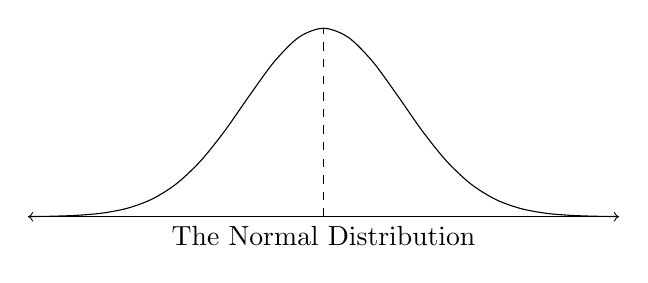
\begin{tikzpicture}[yscale = 6]
					\draw[<->] (-3.75, 0) -- node[below] {The Normal Distribution} ++ (7.5, 0);
					\draw[domain = -3.75:3.75, smooth, variable = \x] plot({\x}, {(e^(-0.5 * \x * \x))/sqrt(2 * pi)});
					\draw[dashed] (0,0) -- (0, 0.399);
				\end{tikzpicture}
			\end{center}
			The \textbf{Normal} distribution (typically denoted $\varphi$) is a density curve that is bell-shaped and symmetrical with inflection points one standard deviation from the mean.\footnote{The Normal distribution is defined as such: \[\varphi(x) = \frac{e^{-x^2/2}}{\sqrt{2\pi}}\]} Its mean and standard deviation are 0 and 1 respectively.\\
			For a curve to be Normal, it must be some transformation\footnote{Changing the mean shifts the graph of the Normal distribution horizontally while changing the standard deviation stretches or shrinks it vertically (the larger, the flatter, and the more data in the \enquote{tails}).} of the Normal distribution curve. A Normal curve with parameters $\mu$ and $\sigma$ is denoted $\mathcal{N}(\mu, \sigma)$, and its application to a variable $X$ is denoted $X\sim\mathcal{N}(\mu,\sigma)$.\footnote{A Normal distribution of $X$ with parameters $\mu$ and $\sigma$can also be denoted as such:\[f(x\mid\mu,\sigma^2) = \frac{1}{\sigma}\varphi\left(\frac{x - \mu}{\sigma}\right)\]} \\
			To justify the Normality of a data set, a modified box plot can be created and symmetry and a lack of variance shown. \\
			Percentile can be found using the \textbf{cumulative Normal distribution function} $\Phi$.\footnote{The cumulative Normal distribution function is defined as such, where $\erf$ is the error function:\[\Phi(x) = \int_{-\infty}^x\varphi(t)\,dt = \frac{1}{2}\left[1 + \erf\left(\frac{x}{\sqrt{2}}\right)\right]\]Percentile can be evaluated on a calculator (for a standard or nonstandard Normal distribution) using the \texttt{normalcdf} (\texttt{2nd/distr/2}) function:\[P(X < x) = \normalCDF{-\infty}{x}{\mu}{\sigma}\]The probability of $X$ falling within a specific range can be found with this function as well:\[P(x_1 < X < x_2) = \normalCDF{x_1}{x_2}{\mu}{\sigma}\]}
			\[\Phi(x) = P(X < x)\]
			The \textbf{inverse Normal function} $\Phi^{-1}$ takes a percentile as an input and returns a value.\footnote{A percentile's corresponding $x$ value can be found using the \texttt{invNorm} (\texttt{2nd/distr/3})function:\[x = \Phi(P(X < x)) = \invNormal{P(X < x)}{\mu}{\sigma}{LEFT}\]}
			\[\Phi^{-1}(P(X < x)) = x\]
			The Normal distribution follows the \textbf{empirical rule}, which states the following:
			\[\footnotesize\begin{array}{|c|ccc|cccc|}\hline
				\rm{Range} & \mu \pm \sigma & \mu \pm 2\sigma & \mu \pm 3\sigma & (\mu, \mu + \sigma) & (\mu + \sigma, \mu + 2\sigma) & (\mu + 2\sigma, \mu + 3\sigma) & (\mu + 3\sigma, \infty)\\\hline
				\text{Proportion of Data} & 60\% & 95\% & 99.7\% & 34\% & 13.5\% & 2.35\% & 0.15\% \\\hline
			\end{array}\]
			\begin{center}
				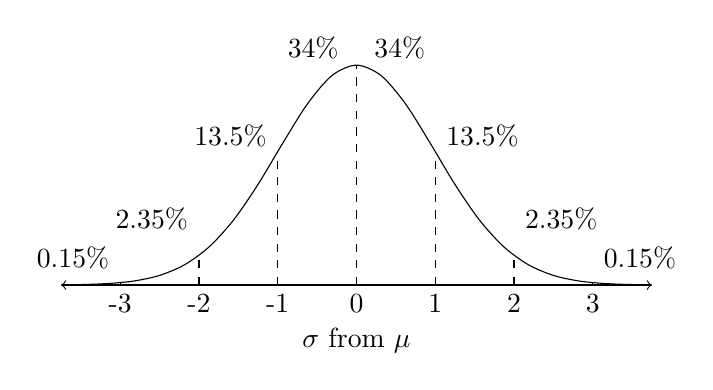
\begin{tikzpicture}[yscale = 7]
					\draw[<->] (-3.75, 0) -- (3.75, 0);
					\draw[domain = -3.75:3.75, smooth, variable = \x] plot({\x}, {e^(-0.5 * \x * \x)/sqrt(2 * pi)});
					\draw[dashed] (0, 0) node[below]{0} -- (0, 0.399);
					\draw[dashed] (-1, 0) node[below]{-1} -- (-1, 0.242);
					\draw[dashed] (1, 0) node[below]{1} -- (1, 0.242);
					\draw[dashed] (-2, 0) node[below]{-2} -- (-2, 0.054);
					\draw[dashed] (2, 0) node[below]{2} --  (2, 0.054);
					\draw[dashed] (-3, 0) node[below]{-3} --  (-3, 0.004);
					\draw[dashed] (3, 0) node[below]{3} --  (3, 0.004);
					\node[] at (-0.55,0.43) {34\%};
					\node[] at (0.55,0.43) {34\%};
					\node[] at (-1.6, 0.27) {13.5\%};
					\node[] at (1.6, 0.27) {13.5\%};
					\node[] at (-2.6, 0.12) {2.35\%};
					\node[] at (2.6, 0.12) {2.35\%};
					\node[] at (-3.6, 0.05) {0.15\%};
					\node[] at (3.6, 0.05) {0.15\%};
					\node[] at (0, -0.1) {$\sigma$ from $\mu$};
				\end{tikzpicture}
			\end{center}
			To simulate a situation that shows Normality, random numbers can be generated following a Normal distribution.\footnote{To generate $n$ random numbers following a Normal distribution, the $\randomnorm$ (\texttt{math/PROB/6}) function can be used as such:\[\randnorm{\mu}{\sigma}{n} = \{x_1, x_2 , \ldots, x_n\}\]This list can then be stored using $\texttt{sto}\to\texttt{L}_n$}
			\subsection*{Standardization and $z$-Scores}
				The $\pmb{z}$\textbf{-score} is the number of standard deviations away from the mean.\footnote{$z$-scores follow the same conventions as variables, $Z$ being used for any value, $z$ for any particular value, and $z_i$ for a defined particular value. The subscript may also denote the variable that it is the $z$-score of, though, in case the cases would correspond, as in $Z_X$, $z_x$, and $z_{x,i}$}
				\[z = \z{x}{\mu}{\sigma}\]
				$z$-scores allow the standard Normal distribution to always be used\footnote{$z$ should be used in place of $x$ when working with $\varphi$ and $\Phi$.}, as it turns $x$ into $z$, $\mu$ into 0 (as the numerator becomes zero), and $\sigma$ into 1 (as $z$ is measured in units of $\sigma$).
				\begin{align*}
					f(x) &= \varphi(z) & F(x) &= \Phi(z)
				\end{align*}
				\callout{17}{$z$-scores can always be calculated, but Normality must be confirmed in order for percentile to be calculable.}
				When answering a question involving calculating the value with a corresponding percentile, the following should be done:
				\begin{enumerate}
					\item Define the variable and its distribution, using the given parameters (and justifying Normality).
					\begin{enumerate}
						\item To show Normality, the situation can be quoted, a modified box plot can be used, or a \textbf{Normal probability plot}, which shows $x$ vs $z$, can be created, and its straightness verified.
						\item If a graph is not given, draw the distribution, labeling the mean, given/desired particular value(s), and given/desired percentiles.
					\end{enumerate}
					\item Calculate/denote the $z$-scores of any particular values.
					\begin{enumerate}
						\item Use the definition of $z$-score as the number of standard deviations from the mean if given particular values.
						\item Use the inverse Normal function if given percentiles.
					\end{enumerate}
					\item Use the formula for $z$-score to calculate the desired variable.
						\begin{align*}
							x &= \mu + z\sigma & \mu &= x - z\sigma & \sigma &= \frac{x - \mu}{z}
						\end{align*}
				\end{enumerate}
	\chapter{One-Variable Categorical Data}
		\textbf{Categorical variables} assign labels that place each individual into one of several groups, while \textbf{quantitative variables} provide values that describe or measure some characteristic. \\
		A \textbf{frequency table} shows the number of individuals that have a certain value while a \textbf{relative frequency table} shows the percentage of all individuals in the data set that have that particular value. \\
		\textbf{Bar graphs} show each category as a bar, the height of which corresponds to its frequency. \\
		\textbf{Pie charts} show each category as some section of a circle that is bounded by two radii. The areas of each slice is proportional to the frequency. \\
\end{document}